% Created 2025-01-11 Sat 00:21
% Intended LaTeX compiler: lualatex
\documentclass[11pt]{article}
\usepackage{fontspec}
\usepackage{graphicx}
\usepackage{lilyglyphs}
\usepackage{graphicx}
\usepackage{longtable}
\usepackage{wrapfig}
\usepackage{rotating}
\usepackage[normalem]{ulem}
\usepackage{amsmath}
\usepackage{amssymb}
\usepackage{capt-of}
\usepackage{hyperref}
\usepackage[cm]{fullpage}
\usepackage[headheight=15pt, headsep=10pt, top=1in, bottom=1in, left=0.75in, right=0.75in]{geometry} % Ensure sufficient header space
\usepackage{fancyhdr}
\pagestyle{fancy}
\fancyhf{}
\fancyhead[L]{\textbf{Master Jazz Standards}} % Left header with title
\fancyhead[R]{\textbf{Bartev -  2025-01}} % Right header with author
\fancyfoot[C]{\thepage}
\fancyfoot[R]{Printed \today} % Right footer with today's date
\renewcommand{\headrulewidth}{0.4pt} % Optional: Add a horizontal rule below the header
\makeatletter
\let\ps@plain\ps@fancy % Apply "fancy" style to the first page
\let\maketitle\relax % Suppress default title/author rendering
\makeatother
\author{Bartev}
\date{2025-01-06}
\title{master-jazz-standards}
\hypersetup{
 pdfauthor={Bartev},
 pdftitle={master-jazz-standards},
 pdfkeywords={},
 pdfsubject={},
 pdfcreator={Emacs 29.4 (Org mode 9.6.15)}, 
 pdflang={English}}
\begin{document}

\maketitle
Here are some thoughts from Nathan Graybeal's YouTube post \href{https://www.youtube.com/watch?v=qdobZsTTbbw\&list=LL}{9 Steps to Mastering Any Jazz Standard}.
\section*{Learn the Melody}
\label{sec:org81af06b}

Serves as the melodic basis of your solo.

Embellish the melody.
\begin{itemize}
\item Change the rhythm
\item Add repeated notes and accents
\item Add extra notes and pitches
\item Improvise over long notes or rests
\end{itemize}
\section*{Learn arpeggios of every chord}
\label{sec:org60ea875}

Learn basic 4 note arpeggios for every chord

\begin{center}
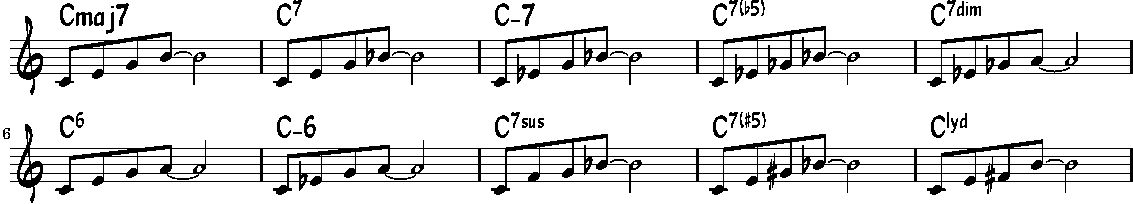
\includegraphics[width=0.98\linewidth]{arpeggios.pdf}
\end{center}

\section*{Try a different permutation}
\label{sec:org676e04e}
Rearrange the order of the chord tones.

\begin{center}
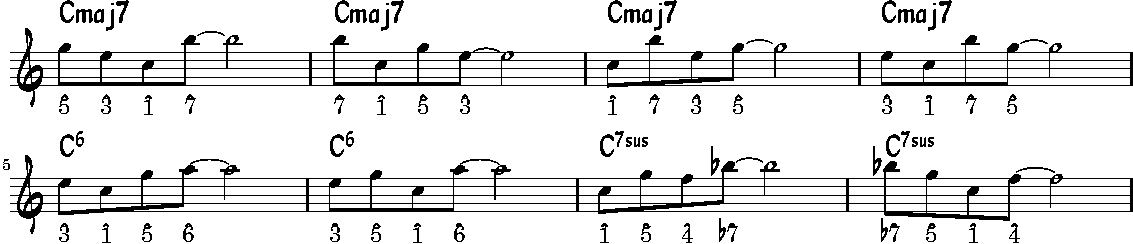
\includegraphics[width=0.98\linewidth]{permute-arpeggio.pdf}
\end{center}
\section*{Add 9th to the arpeggios}
\label{sec:org59a9eb6}

Create a constrant stream of 8th notes

\begin{center}
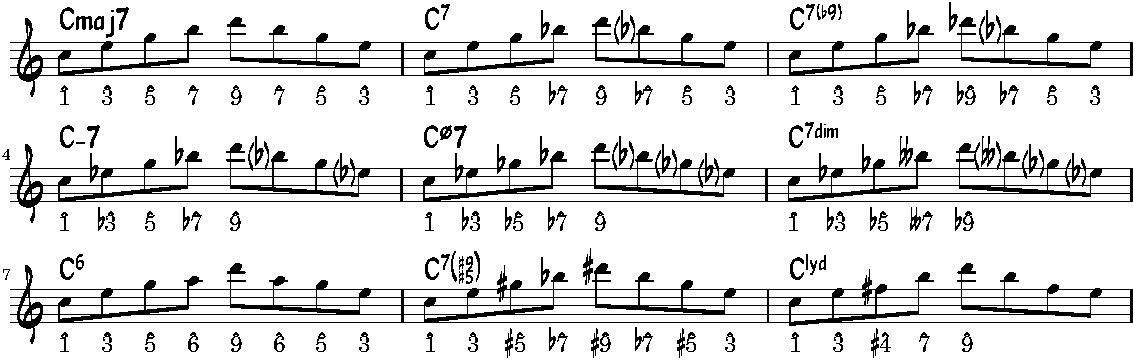
\includegraphics[width=0.98\linewidth]{arpeggeio-to-9th.pdf}
\end{center}

\subsection*{Four Rules to remember}
\label{sec:org291e153}
\subsubsection*{Half dim chord}
\label{sec:org461150d}
\begin{itemize}
\item \flat9 is an avoid tone
\item \natural9 is a color tone
\item Just play the root at the top

So, in a minor ii-v-i, we'd have

\begin{center}
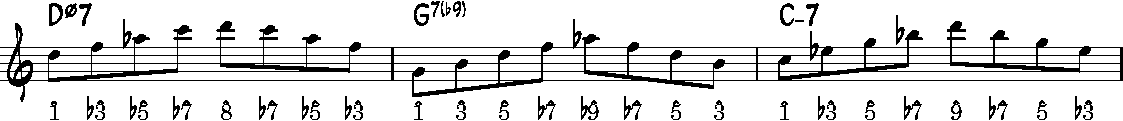
\includegraphics[width=0.98\linewidth]{arpeg-9th-half-dim.pdf}
\end{center}
\end{itemize}

\subsubsection*{Diminished chord}
\label{sec:org787d373}

The diminished chord comes from the diminished scale (whole/half dim).

\begin{center}
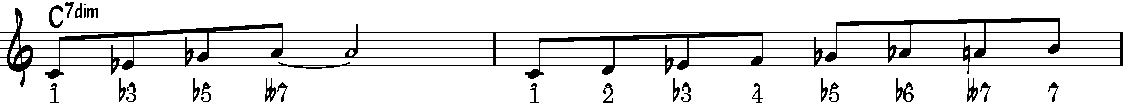
\includegraphics[width=0.98\linewidth]{diminished-scale-and-arpeg.pdf}
\end{center}

In this case, just go up to the root again.

\begin{center}
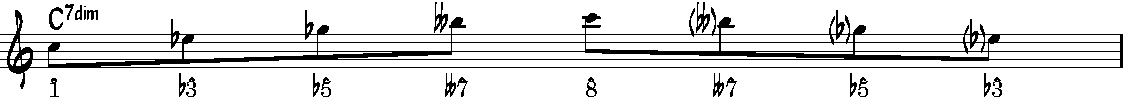
\includegraphics[width=0.98\linewidth]{arpeg-9th-dim.pdf}
\end{center}

\subsubsection*{Minor 7 chords that are functioning as iii-7 chords}
\label{sec:org2bc1f0e}
\begin{itemize}
\item In this case, you should also go up to the root, not the 9th
\end{itemize}
\subsubsection*{Chords that only last 2 beats}
\label{sec:orgb85709b}
\begin{itemize}
\item In this case, only arpeggiate up 4 notes since that's all we have time for.
\end{itemize}
\end{document}
